\documentclass[aspectratio=43]{beamer}
\usepackage[latin1]{inputenc}
\usepackage{amsmath}
\usepackage{amsfonts}
\usepackage{amssymb}
\usepackage{makeidx}
\usepackage{graphicx}
\usepackage{array}

% Customization
\mode<presentation>{
	\usetheme{CambridgeUS}
	\usecolortheme{dolphin}
	\setbeamertemplate{navigation symbols}{}
}

% Define colors
\definecolor{darkgreen}{rgb}{0.0, 0.5, 0.13}
\definecolor{darkblue}{rgb}{0.0, 0.0, 0.55}
\definecolor{darkred}{rgb}{0.55, 0.0, 0.0}

% Title and author
\title[Perturbative QCD predictions for Higgs production]{pQCD predictions for Higgs production}
\author{\textbf {Jes\'us Urtasun Elizari}}
%\institute{\textbf {University of Milan}}
\date{Milan, December 2020}

\begin{document}

% Front slide
\begin{frame}

	%\maketitle
	\vspace{1.0 cm}
	
	\center{\color{blue}High precision perturbative QCD predictions \\ for Higgs boson production at the LHC}
	
	\vspace{0.25 cm}
	\center{Jes\'us Urtasun Elizari}
	\center{Milan, December 2020}

	\begin{figure}
		\minipage{1\textwidth}
		
\includegraphics[width = 3.0 cm]{plots/unimi.png}
		\hfill
		
\includegraphics[width = 3.0 cm]{plots/n3pdf.png}
		\hfill
		
\includegraphics[width = 3.0 cm]{plots/erc.png}
		\endminipage
	\end{figure}

	\vspace{1.0 cm}
	
	{\scriptsize \color{blue} This project has received funding from the European Union$'$s Horizon 2020 research and innovation program under grant agreement No 740006.}

\end{frame}

% Introduction
\begin{frame}

	\frametitle{Outline}
	
	\begin{enumerate}
		\item {\color{blue}QCD and collider physics}
		\begin{itemize}
			\item QCD Factorization
			\item Partonic cross section and perturbative QCD
		\end{itemize}
		\item {\color{blue}The N3PDF project}
		\begin{itemize}	
			\item Parton Distribution Functions
			\item Machine Learning for PDFs
		\end{itemize}	
		\item {\color{blue}All order perturbative resummation}
		\begin{itemize}
			\item Higher orders radiative corrections
			\item Resummation of large logarithmic corrections
		\end{itemize}
		\item {\color{blue}Precise and fast predictions for Higgs boson physics}
		\begin{itemize}
			\item Higgs production at the LHC
			\item HTurbo numerical code
			\item Preliminary results $\&$ Conclusions
		\end{itemize}
	\end{enumerate}
	
\end{frame}

% QCD in a nutshell
\begin{frame}

	\center{\color{blue}QCD and collider physics}

\end{frame}

% LHC physics
\begin{frame}

	\frametitle{QCD}
	\framesubtitle{LHC physics}
	
	\begin{figure}
		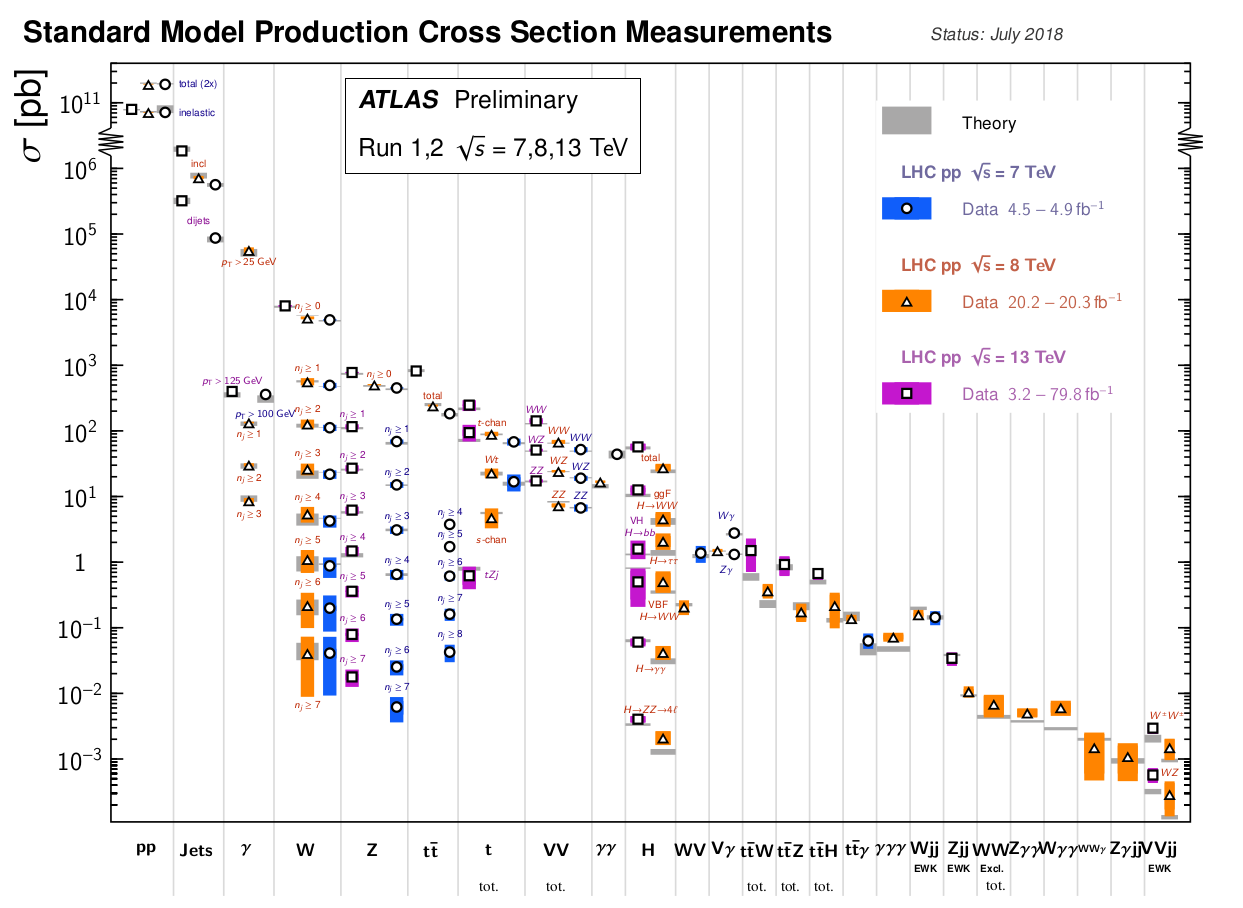
\includegraphics[width = 9.5 cm]{plots/section1/lhc_measurements.png}
	\end{figure}

\end{frame}

% Factorization theorem
\begin{frame}

	\frametitle{QCD}
	\framesubtitle{Factorization theorem}

	\vspace{0.4 cm}
	
	\begin{figure}
		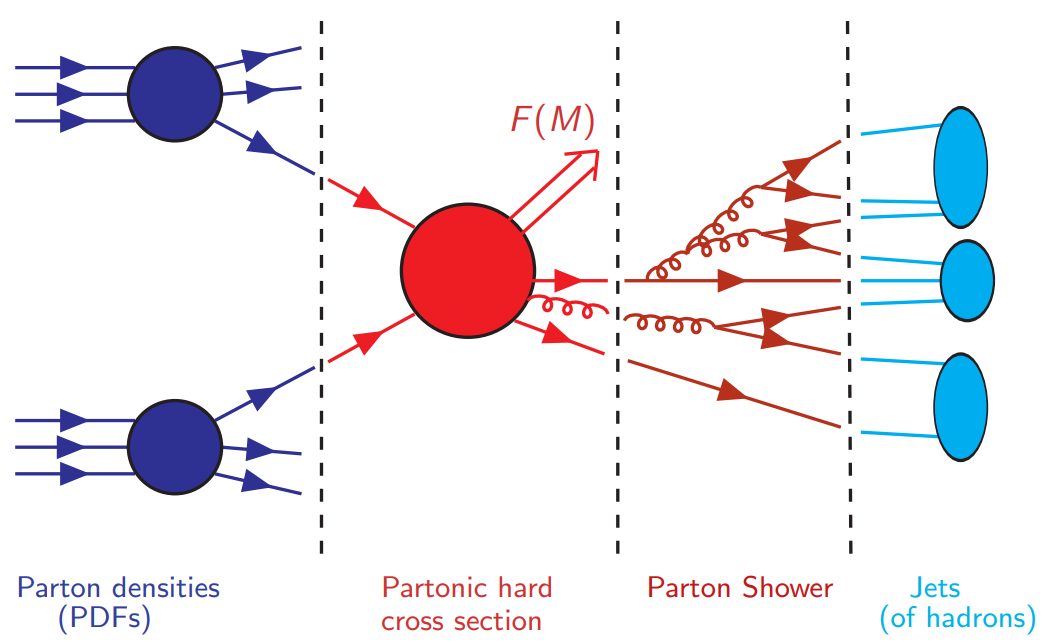
\includegraphics[width = 7 cm]{plots/section1/factorization_1.png}
	\end{figure}
	
	Compute hadronic cross sections is a {\color{red}hard problem} $\longrightarrow$ {\color{blue} QCD Factorization}
	
	\begin{equation}
		\sigma^{\textrm{F}}(p_{1}, p_{2}) =
		\int_{0}^{1} dx_{1} dx_{2} \; {\color{blue} f_{\alpha}(x_{1}, \mu_{F}^{2}) \ast f_{\beta}(x_{2}, \mu_{F}^{2})}
		\; \ast \;  
		{\color{red}\hat{\sigma}^{\textrm{F}}_{\alpha \beta}(x_{1}p_{1}, x_{2}p_{2}, \alpha_{s}(\mu_{R}^{2}), \mu_{F}^{2})} \nonumber
	\end{equation}

\end{frame}

% Partonic cross section
\begin{frame}
	
	\frametitle{QCD}
	\framesubtitle{Partonic cross section}
	
	\begin{figure}
		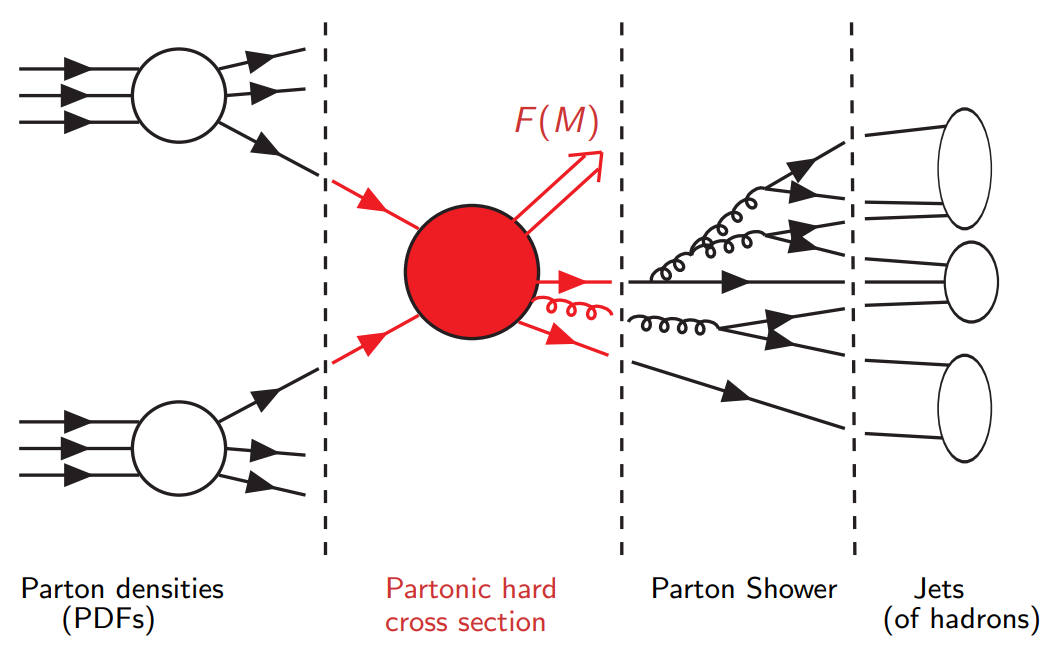
\includegraphics[width = 7 cm]{plots/section1/factorization_2.png}
	\end{figure}
	
	\begin{itemize}
		\item Parton densities (PDFs) ${\color{blue} f_{\alpha}(x_{i}, \mu_{F}^{2})}$: non perturbative but universal
		\item Partonic cross section {\color{red}$\hat{\sigma}^{\textrm{F}}_{\alpha \beta}$}: process dependent but computable as perturbative series in $\alpha_{s}$
	\end{itemize}
	
\end{frame}

% Perturbative QCD
\begin{frame}

	\frametitle{QCD}
	\framesubtitle{Perturbative QCD}
	
	\begin{columns}
		
		\column{0.45\textwidth}
		
		\begin{itemize}
			\item Born cross section is the leading-order (LO) term of the perturbative series
			\item $\sigma^{(1)}, \sigma^{(2)}, \sigma^{(3)}$ are the NLO, NNLO, N3LO corrections
		\end{itemize}
		
		\column{0.45\textwidth}
		\begin{figure}[!htb]
			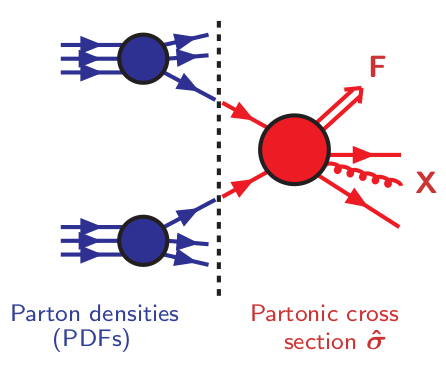
\includegraphics[width = 5 cm]{plots/section1/factorization_3.png}
		\end{figure}
	
	\end{columns}
	
	\begin{equation}
		\hat{\sigma} = \sigma^{\texttt{Born}} \Big( 1 +
		\alpha_{s} \sigma^{(1)} + 
		\alpha_{s}^{2} \sigma^{(2)} + 
		\alpha_{s}^{3} \sigma^{(3)} + ... \Big) \nonumber
	\end{equation}
	
	Lower order predictions strongly depend on the auxiliary and unphysical renormalization and factorization scales $\longrightarrow$ {\color{red}Need higher order corrections to increase theoretical accuracy!}

\end{frame}

% The N3PDF project
\begin{frame}

	\center{\color{blue}The N3PDF project}

\end{frame}

% The N3PDF project
\begin{frame}

	\begin{figure}
		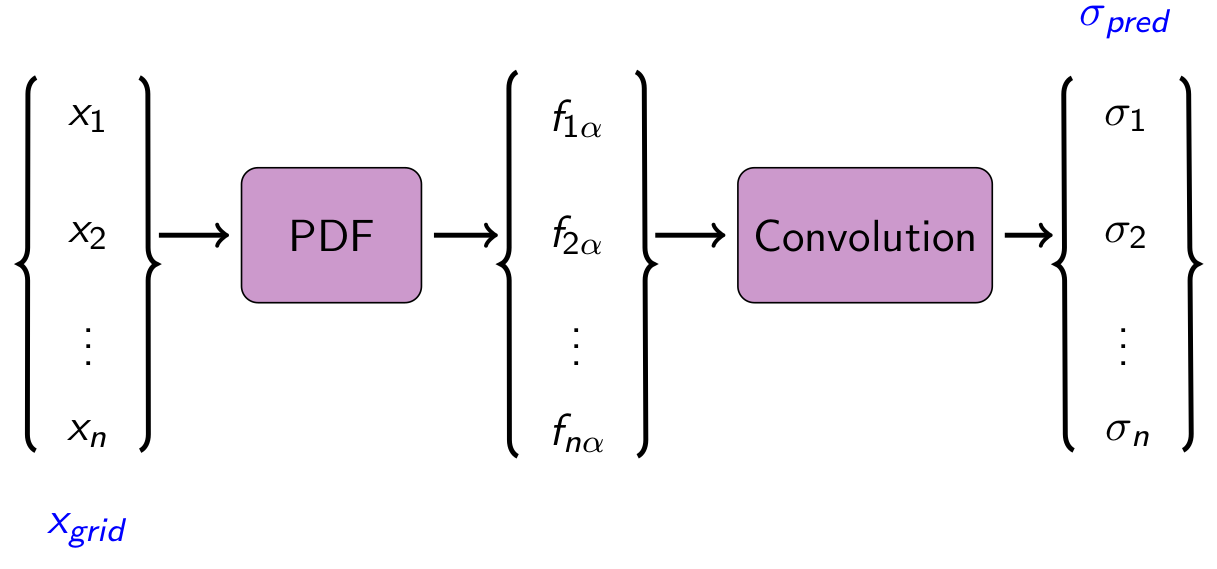
\includegraphics[width = 8.5 cm]{plots/section2/TF_convolution.png}
	\end{figure}

\end{frame}

% The N3PDF project
\begin{frame}

	\begin{figure}
		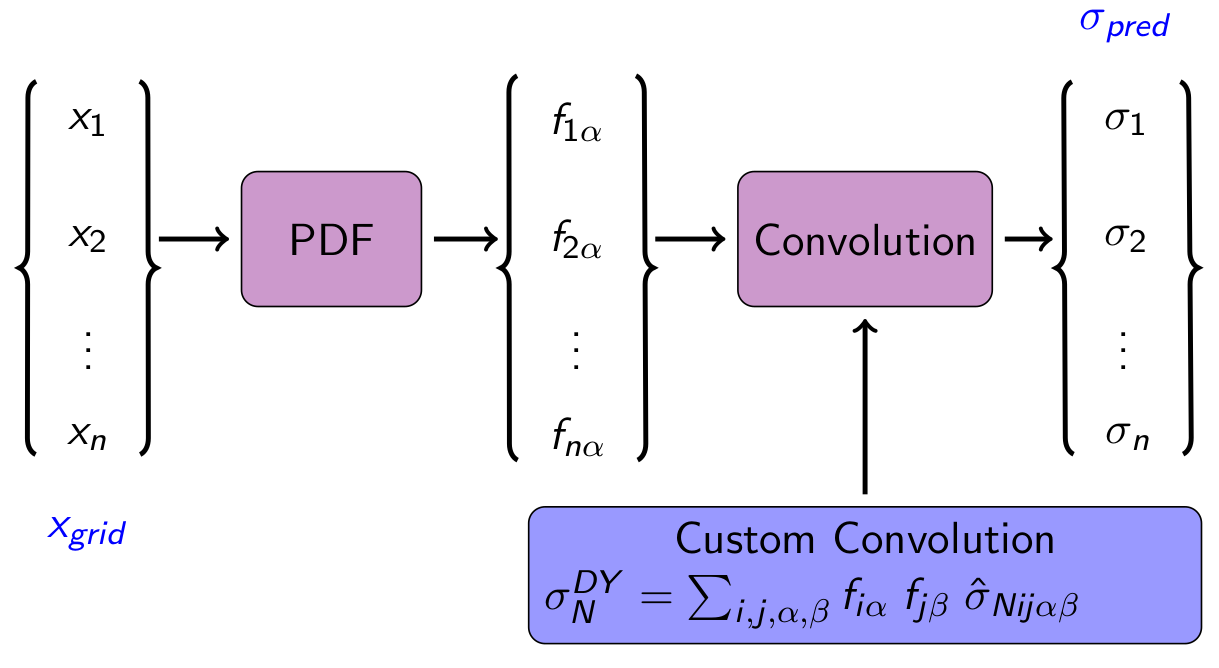
\includegraphics[width = 8.5 cm]{plots/section2/TF_convolution2.png}
	\end{figure}

\end{frame}

% Results DIS ratio
\begin{frame}

	\frametitle{Results}
	\framesubtitle{Checking computation}
	
	{\Large DIS:}
	\begin{table}
		\centering
		\begin{tabular}{c c c c}
			& TensorFlow & Custom & Ratio \\ \hline
			& 1.9207904 & 1.9207904 & {\color{darkgreen} 1.0000000} \\
			Convolution & 2.4611666 & 2.4611664 & {\color{darkgreen} 0.9999999} \\
			& 1.3516952 & 1.3516952 & {\color{darkgreen} 1.0000000} \\
			\hline
			& 1.8794115 & 1.8794115 & {\color{darkgreen} 1.0000000} \\
			Gradient & 1.505316 & 1.505316 & {\color{darkgreen} 1.0000000} \\
			& 2.866085 & 2.866085 & {\color{darkgreen} 1.0000000} \\
			\hline
		\end{tabular}
	\end{table}

\end{frame}

% Results hadronic ratio
\begin{frame}
	
	\frametitle{Results}
	\framesubtitle{Checking computation}
	
	{\Large Hadronic:}
	\begin{table}
		\centering
		\begin{tabular}{c c c c}
			& TensorFlow & Custom & Ratio \\ \hline
			& 8.142365 & 8.142366 & {\color{darkgreen} 1.0000001} \\
			Convolution & 8.947762 & 8.947762 & {\color{darkgreen} 1.0000000} \\
			& 7.4513326 & 7.4513316 & {\color{darkgreen} 0.9999999} \\
			\hline
			& 18.525095 & 18.525095 & {\color{darkgreen} 1.0000000} \\
			Gradient & 19.182995 & 19.182993 & {\color{darkgreen} 0.9999999} \\
			& 19.551006 & 19.551004 & {\color{darkgreen} 0.9999999} \\
			\hline
		\end{tabular}
	\end{table}

\end{frame}

% Results memory
\begin{frame}

	\frametitle{Results}
	\framesubtitle{Memory saving}
	
	{\Large Hadronic only:}
	\begin{table}
		\centering
		\begin{tabular}{c c c c}
			& TensorFlow & Custom Convolution & Diff \\ \hline
			Virtual & {\color{red} 17.7 GB} & {\color{darkgreen} 13.8 GB} & {\color{darkgreen} 3.9 GB} \\
			RES & {\color{red} 12.1 GB} & {\color{darkgreen} 8.39 GB} & {\color{darkgreen} 3.2 GB} \\ \hline
		\end{tabular}
	\end{table}
	
	\hfill
	
	{\Large Global:}
	\begin{table}
		\centering
		\begin{tabular}{c c c c}
			& TensorFlow & Custom Convolution & Diff \\ \hline
			Virtual & {\color{red} 23.5 GB} & {\color{darkgreen} 19.7 GB} & {\color{darkgreen} 3.8 GB} \\
			RES & {\color{red} 18.4 GB} & {\color{darkgreen} 12.5 GB} & {\color{darkgreen} 5.9 GB} \\ \hline
		\end{tabular}
	\end{table}
	
	{\color{blue}"Towards hardware acceleration for parton densities estimation",\\ https://arxiv.org/abs/1909.10547}

\end{frame}

% All orders perturbative resummation
\begin{frame}

	\center{\color{blue}All orders perturbative resummation}

\end{frame}

% Higher order corrections
\begin{frame}

	\frametitle{Resummation in QCD}
	\framesubtitle{Higher order corrections}
	\begin{columns}
	
	\column{0.5\textwidth}
	
	\begin{enumerate}
		\item Calculation of higher order corrections is {\color{red}not an easy task} due to {\color{red} infrared (IR) soft and collinear singularities}
		\item Final state singularities {\color{blue}cancel} by combining real and virtual contributions
		\item Initial state collinear singularities {\color{blue}factorized} inside the PDFs
	\end{enumerate}
	
	\column{0.45\textwidth}
	\begin{figure}[!htb]
		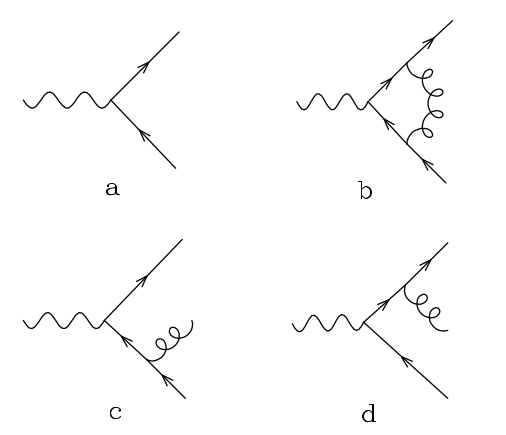
\includegraphics[width = \linewidth]{plots/qcd_corrections.png}
	\end{figure}
	
	\end{columns}

\end{frame}

% qT resummation I
\begin{frame}

	\frametitle{Resummation in QCD}
	\framesubtitle{$q_{\perp}$ resummation}
	
	\begin{columns}
	
		\column{0.55\textwidth}
		
		\center	Study the differential $q_{\perp}$ distribution \\
		\center	$h_{1}(p_{1}) + h_{2}(p_{2}) \longrightarrow F(M, {\color{red}q_{\perp}}) + X$
	
		\column{0.45\textwidth}
		
		\begin{figure}
			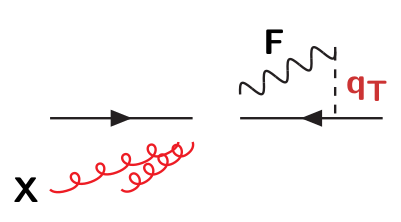
\includegraphics[width = 4cm]{plots/qT_diagram.png}
		\end{figure}

	\end{columns}

	$\int_{0}^{Q_{\perp}^{2}} \; dq_{\perp}^{2} \frac{d\hat{\sigma}}{dq_{\perp}^{2}} \sim c_{0} + \alpha_{s}(c_{12}L^{2} + c_{11}L + c_{10}) + ..., \textrm{\quad where \quad} L = \ln (q_{\perp} / M^{2})$

	\begin{figure}
		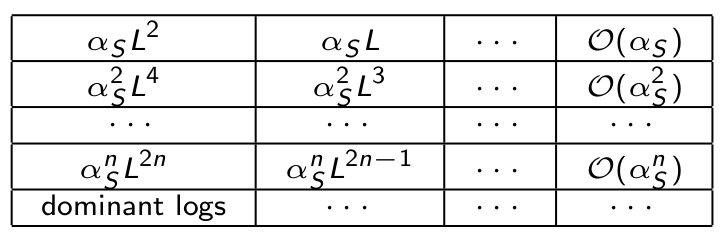
\includegraphics[width = 7.5cm]{plots/qT_logs_table.png}
	\end{figure}

	Truncated fixed order predictions $\rightarrow$ {\color{red}enhanced $\alpha_{s}^{n}\ln^{m}(M^{2}/q_{\perp}^{2})$ appear}

\end{frame}

% Resummation in QCD II
\begin{frame}

	\frametitle{Resummation in QCD}
	\framesubtitle{$q_{\perp}$ resummation}

	Separate partonic $q_{\perp}$ distribution as follows
	
	\begin{equation}
		\frac{d\hat{\sigma}_{ab}}{dq_{\perp}^{2}} =
		\Bigg[ \frac{d\hat{\sigma}^{\textrm{(res.)}}_{ab}}{dq_{\perp}^{2}} \Bigg]_{\textrm{l.a.}} + 
		\Bigg[ \frac{d\hat{\sigma}^{\textrm{(fin.)}}_{ab}}{dq_{\perp}^{2}} \Bigg]_{\textrm{f.o.}} \textrm{\quad, \quad such that} \nonumber
	\end{equation}

	\begin{align}
		\int_{0}^{q_{\perp}^{2}} dq_{\perp}^{2} \frac{d\hat{\sigma}^{\textrm{(res.)}}_{ab}}{dq_{\perp}^{2}} \sim & \sum \alpha_{s}^{n} \log^{m} \frac{M^{2}}{q_{\perp}^{2}} \textrm{\quad for \quad} q_{\perp} \rightarrow 0 \nonumber \\
		\lim_{q_{\perp} \rightarrow 0}\int_{0}^{q_{\perp}^{2}} dq_{\perp}^{2} \frac{d\hat{\sigma}^{\textrm{(fin.)}}_{ab}}{dq_{\perp}^{2}} &= 0 \nonumber 
	\end{align}

	Resummed and finite components can be matched (LL+LO, NLL+NLO, NNLO+NNLL, ...) to have uniform accuracy in a wide range of $q_{\perp}$
\end{frame}

% qT resummation III
\begin{frame}

	\frametitle{Resummation in QCD}
	\framesubtitle{$q_{\perp}$ resummation}
	
	Resummation holds in impact parameter space $b$
	\begin{equation}
		\frac{d\hat{\sigma}_{ab}^{\textrm{(res.)}}}{dq_{\perp}^{2}} = \frac{M^{2}}{\hat{s}} \int db \; \frac{b}{2} \; J_{0}(b q_{\perp}) \; {\color{red} \mathcal{W}_{ab}(b, M)} \nonumber
	\end{equation}
	
	with ${\color{red}\mathcal{W}_{ab}}$ also expressed in Mellin space (with respect to $z = M^{2}/\hat{s}$)
	\begin{equation}
		{\color{red} \mathcal{W}_{N}(b, M) = \mathcal{H}_{N}(\alpha_{s}) \times \exp\{\mathcal{G}_{N}(\alpha_{s}, L)\}} \quad\textrm{being}\quad L \equiv \log(M^{2}b^{2}) \nonumber
	\end{equation}

	\begin{itemize}
		\item Large logarithms exponentiated in the universal Sudakov form factor {\color{red}$\mathcal{G}_{N}(\alpha_{s}, L)$}
		\item Constant (b-independent) terms factorized in the process dependent hard factor {\color{red}$\mathcal{H}_{N}(\alpha_{s})$}
	\end{itemize}

	
\end{frame}

% HTurbo
\begin{frame}

	\center{\color{blue}Precise and fast predictions for Higgs boson physics}

\end{frame}

% HqT and HRes
\begin{frame}

	\frametitle{HqT and HRes}
	\framesubtitle{Predictions for Higgs $q_{\perp}$ distribution}
	
	\begin{columns}
		
		\column{0.5\textwidth}
			
		\begin{itemize}
			\item $q_{\perp}$ resummation implemented in numerical codes HqT and HRes {\color{blue}[Catani, de Florian, Ferrera, Grazzini, Tommasini]} 
			\item Higher order accuracy require {\color{red}high computation times}
			\item Codes producing fast and accurate predictions are needed for precision era of the LHC
		\end{itemize}

		\column{0.55\textwidth}
	
		\begin{figure}
			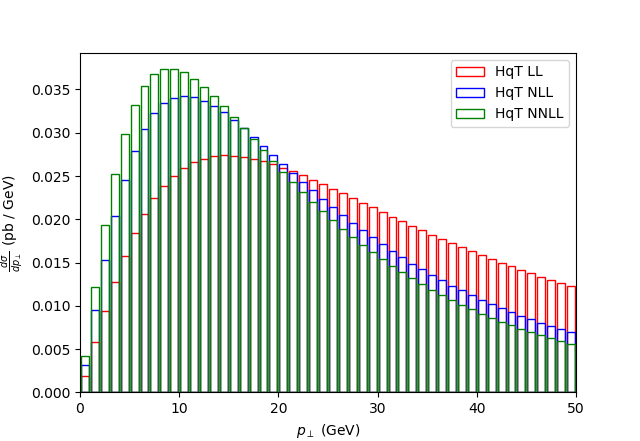
\includegraphics[width = 7 cm]{plots/higgs_qt_all.png}
		\end{figure}		
			
	\end{columns}

\end{frame}

% DYturbo I
\begin{frame}

	\frametitle{HTurbo}
	\framesubtitle{Starting point DYTurbo}

	Numerical code \textbf{DYTurbo} {\color{blue}[Camarda et al.]} ref. at {\color{blue} \href{https://arxiv.org/abs/1910.07049}{1910.07049}}, fast and precise $q_{\perp}$ resummation and several improvements for Drell-Yan ($h_{1}h_{2} \rightarrow V + X \rightarrow l^{+}l^{-} + X$) 
	
	\begin{itemize}
		\item {\color{red}First goal}: set up a numerical code for Higgs boson production starting from  \textbf{DYTurbo}
		\item Set LO amplitude $gg \rightarrow H$
		\item Set Sudakov and Hard coefficients for Higgs production
		\item Compare with \textbf{HRes} and \textbf{HqT}
	\end{itemize}

	\vspace{0.5 cm}

	{\color{red}Final goal}: extend theoretical accuracy up to N$^{3}$LL+N$^{3}$LO

\end{frame}

% DYturbo II
\begin{frame}

	\frametitle{HTurbo}
	\framesubtitle{Starting point DYTurbo}

	\begin{align}
		\mathcal{G}_{N}(\alpha_{s}, L) &= L\;g^{(1)}(\alpha_{s}L) + g^{(2)}(\alpha_{s}L) + \frac{\alpha_{s}}{\pi}g^{(3)}(\alpha_{s}L) + ... \nonumber \\
		\mathcal{H}_{N}(\alpha_{s}) &= 1 + \alpha_{s}\mathcal{H}^{(1)} + \alpha_{s}^{2}\mathcal{H}^{(2)} + ...  \nonumber
	\end{align}
	
	\begin{columns}
		
		\column{0.45\textwidth}

		\begin{align}
			&\textrm{LL} (\sim \alpha_{s}^{n}L^{n+1}): g^{(1)}, \hat{\sigma}^{(0)} \nonumber \\
			&\textrm{NLL} (\sim \alpha_{s}^{n}L^{n}): g^{(2)}, \mathcal{H}^{(1)} \nonumber \\
			&\textrm{NNLL} (\sim \alpha_{s}^{n}L^{n-1}): g^{(3)}, \mathcal{H}^{(2)} \nonumber
		\end{align}
	
		\column{0.45\textwidth}
		
		Start by building predictions up to NNLO+NNLL, then add {\color{blue}N$^{3}$LO+N$^{3}$LL}
		
	\end{columns}

\end{frame}

% Results LL
\begin{frame}
	
	\frametitle{Results}
	\framesubtitle{Comparison HTurbo and HqT - LL}
	
	\begin{figure}
		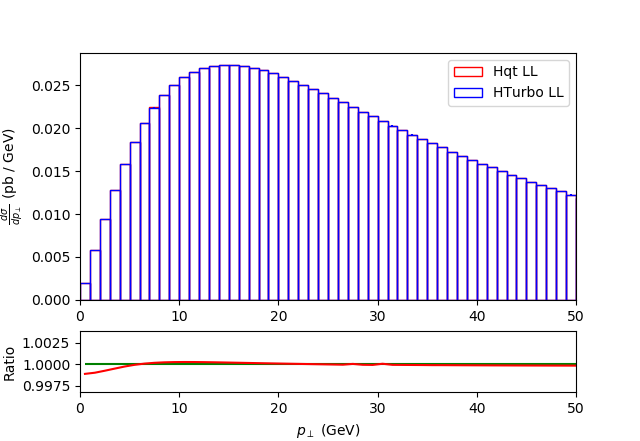
\includegraphics[width = 8cm]{plots/hturbo_LL.png}
	\end{figure}
	
	\begin{itemize}
		\item HTurbo $q_{\perp}$ distribution vs HRes and HqT at LL
		\item Excellent numerical agreement up to the $0.1\%$ level
	\end{itemize}

\end{frame}

% Results NLL
\begin{frame}

	\frametitle{Results}
	\framesubtitle{Comparison HTurbo and HqT - NLL}
	
	\begin{figure}
		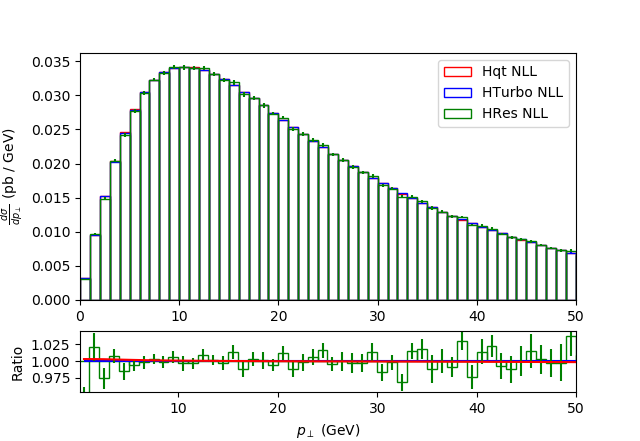
\includegraphics[width = 8cm]{plots/hturbo_NLL.png}
	\end{figure}
	
	\begin{itemize}
		\item HTurbo $q_{\perp}$ distribution vs HRes and HqT at NLL
		\item Excellent numerical agreement up to the $0.1\%$ level
	\end{itemize}

\end{frame}

% Results NNLL
\begin{frame}

	\frametitle{Results}
	\framesubtitle{Comparison HTurbo and HqT - NNLL}
	
	\begin{figure}
		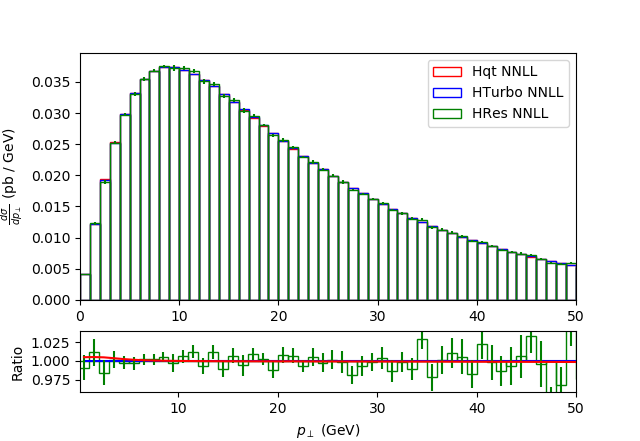
\includegraphics[width = 8cm]{plots/hturbo_NNLL.png}
	\end{figure}
	
	\begin{itemize}
		\item HTurbo $q_{\perp}$ distribution vs HRes and HqT at NNLL
		\item Excellent numerical agreement up to the $0.1\%$ level
\end{itemize}

\end{frame}

% Results all
\begin{frame}
	
	\frametitle{Results}
	\framesubtitle{Comparison HTurbo and HqT - all orders}
	
	\begin{figure}
		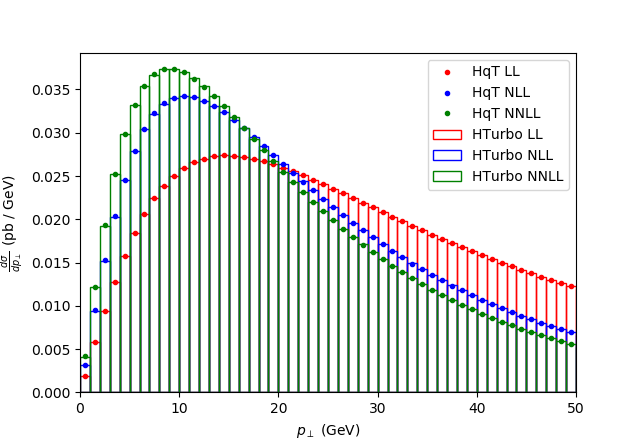
\includegraphics[width = 8cm]{plots/hturbo_all_orders.png}
	\end{figure}
	
	\begin{itemize}
		\item Higher orders lead to more accurate predictions {\color{darkgreen}$\checkmark$} 
		\item Agreement up to NNLL $\longrightarrow$ {\color{blue}ready for N$^{3}$LL}
	\end{itemize}

\end{frame}

% Conclusions
\begin{frame}
	
	\frametitle{Summary $\&$ Conclusions}

	\vspace{2.0 cm}
	
	\begin{enumerate}
		\item Fast and accurate predictions are required towards the precision era of the LHC
		\item Developing a novel numerical code, \textbf{HTurbo}, which implements $q_{\perp}$ resummation for Higgs boson production
		\item HTurbo is {\color{blue} faster than any of the existing codes}
		\item Next steps: 
		\begin{itemize}
			\item Validate results at NNLO
			\item Add {\color{blue}N$^{3}$LO} prediction
			\item Perform phenomenological studies comparing with LHC data
		\end{itemize}

	\end{enumerate}

	\vspace{2.0 cm}

\end{frame}

% Conclusions
\begin{frame}

	\center {\color{blue}Thank you!}

	\begin{figure}
		
\includegraphics[width = 4 cm]{plots/thinking.png}
	\end{figure}		

	{\small \color{blue} This project has received funding from the European Union$'$s Horizon 2020 research and innovation program under grant agreement No 740006.}

\end{frame}


\end{document}